\section{Temporal Data Visualization}\label{sec:temporal-data-visualization}

Temporal data visualization techniques help us visualize a certain change over time.
We can focus on an object, or a set of objects, and try to understand their changes during time.
There are many examples of temporal visualization charts of which the most common are line graphs, bar charts,
Gantt charts, stacked area charts, and even the one we have seen in \Cref{fig:figure2.4}, the Nightingale’s
polar area chart, also known as the Rose chart.

One of the earliest examples worth mentioning is the area chart by William Playfair. He was a Scottish engineer
known for inventing statistical graphs such as bar charts, line graphs of economic data, pie charts, and circle
graphs~\citep{friendly2001milestones}. This chart shows the trade balance of exports and imports to and from Denmark and
Norway from 1700 to 1780.

\begin{figure}[hbt!]
    \begin{center}
        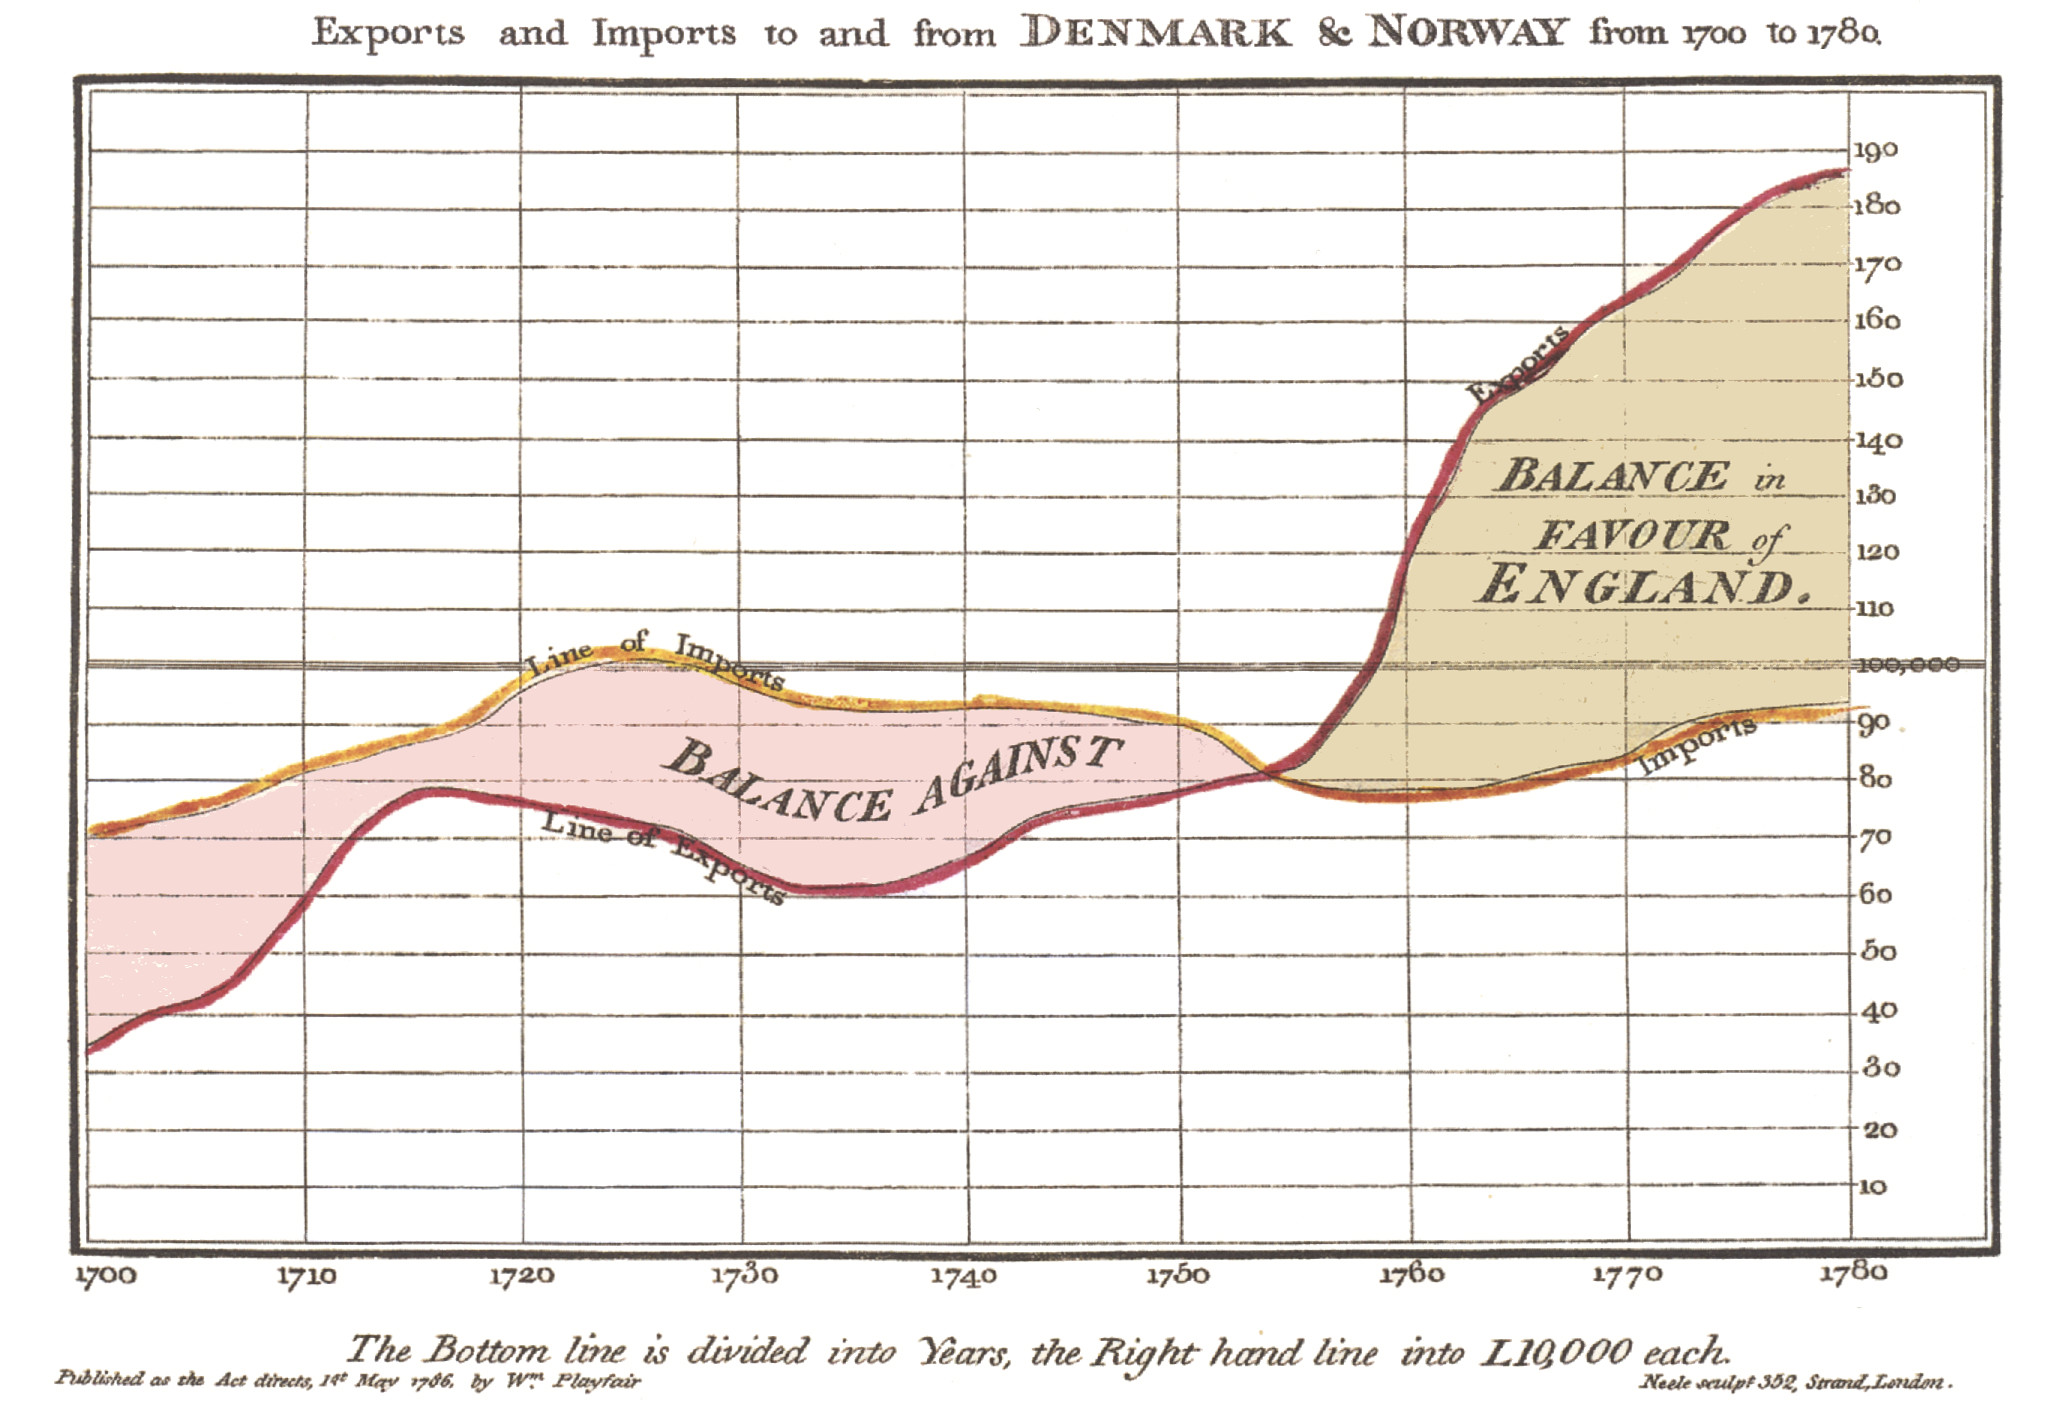
\includegraphics[width=0.7\textwidth]{graphics/2-literature-review/5}
    \end{center}
    \caption{William Playfair's time-series area chart~\citep{playfair1801commercial}}
    \label{fig:figure2.5}
\end{figure}

Aigner et al.~\citep{aigner2007visualizing} provide a number of examples of temporal data visualizations:

\begin{figure}[hbt!]
    \begin{center}
        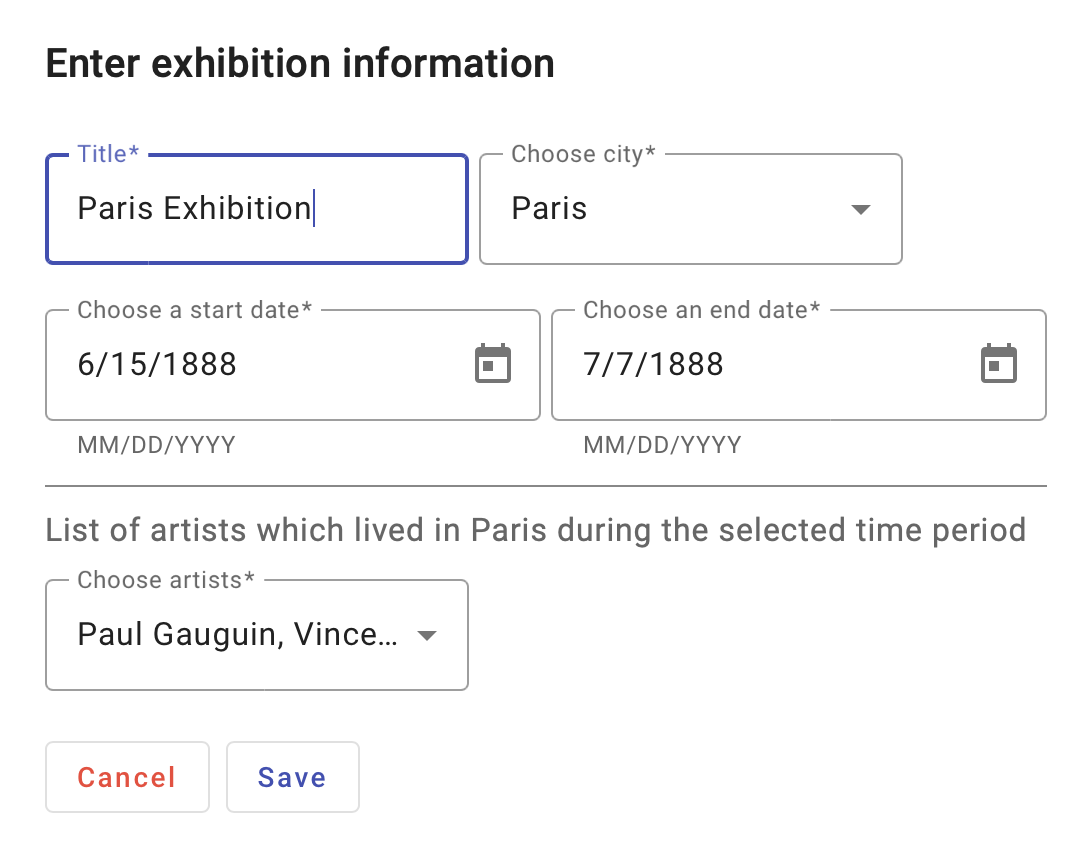
\includegraphics[width=\textwidth]{graphics/2-literature-review/6}
    \end{center}
    \caption{Temporal data visualization examples}
    \label{fig:figure2.6}
\end{figure}

a) animated flow visualization~\citep{van2002image}: smooth animations created from streamline images;
b) feature and event based flow visualization~\citep{reinders2001visualization}: animated visualization based on data abstraction and iconic representations;
c) ThemeRiver~\citep{havre2002themeriver}: static representation of thematic changes in document collections;
d) TimeWheel~\citep{tominski2004axes}: axes-based visualization of multivariate data with focus on temporal dependencies;
e) helix glyphs on maps~\citep{tominski20053d}: emphasis of cyclic patterns in spatio–temporal human health data;
f) flocking boids~\citep{moere2004time}: stock market visualization based on simulation and animation of flocking behavior;
g) cluster and calendar based visualization~\citep{van1999cluster}: visualization of univariate time series on different levels of aggregation;
h) PlanningLines~\citep{aigner2005planninglines}: visualization of project plans with temporal uncertainty; and
i) SimVis~\citep{doleisch2004case}: larger system that combines several views to facilitate flow visualization.